%\subsection{Database Structure}
\label{sec:databasestructure}

We distinguish between two parts of the database, the login part, and the model part. 
The model part is created from our Model \ref{sub:modelComponent} using the ADO.NET Entity Framework(EF) which is described in subsection \ref{sub:adonet}. 
We choose to use ADO.NET EF because then we do not have to worry about converting our tuples to objects and to make sure that changed properties are mapped to the database correctly.  

To administrate users we use the built in ASP.NET membership provider which provides a login system with support for role authorization. 
We use this provider since it saves time instead of building our own login system. 
The major disadvantage is that including the membership providers database scheme with the model is not supported and does not work properly, therefore we had to add a person entity and change the register functionality to also save the registered person in our person table. 
This gives some redundant data, but only the username and email. 

When we need to access data from the membership tables we have to use SQL statements and not the object oriented approached we used for the rest. 
This is limited since our main functionality depends on the model. 

\section{Model Designer}
To administrate the model, we use the Visual Studio inbuilt tool, ADO.NET Entity Model Designer. This tool can create a database from the model, but also generate the model from the database. We generate our database from the model. If any changes is made it is easy to update both the model and the database. 
Our model as it is seen in the ADO.NET Entity Model Designer is shown on figure \ref{fig:edmxModel}.

The lines between the entities represents relations. If it is a many to many relation, the needed relationship table is created behind the scenes. This means the created database actually contains several tables more than entities. To use the relations the navigation properties is used. \vspace{2mm}

\begin{figure}[H]
	\centering
		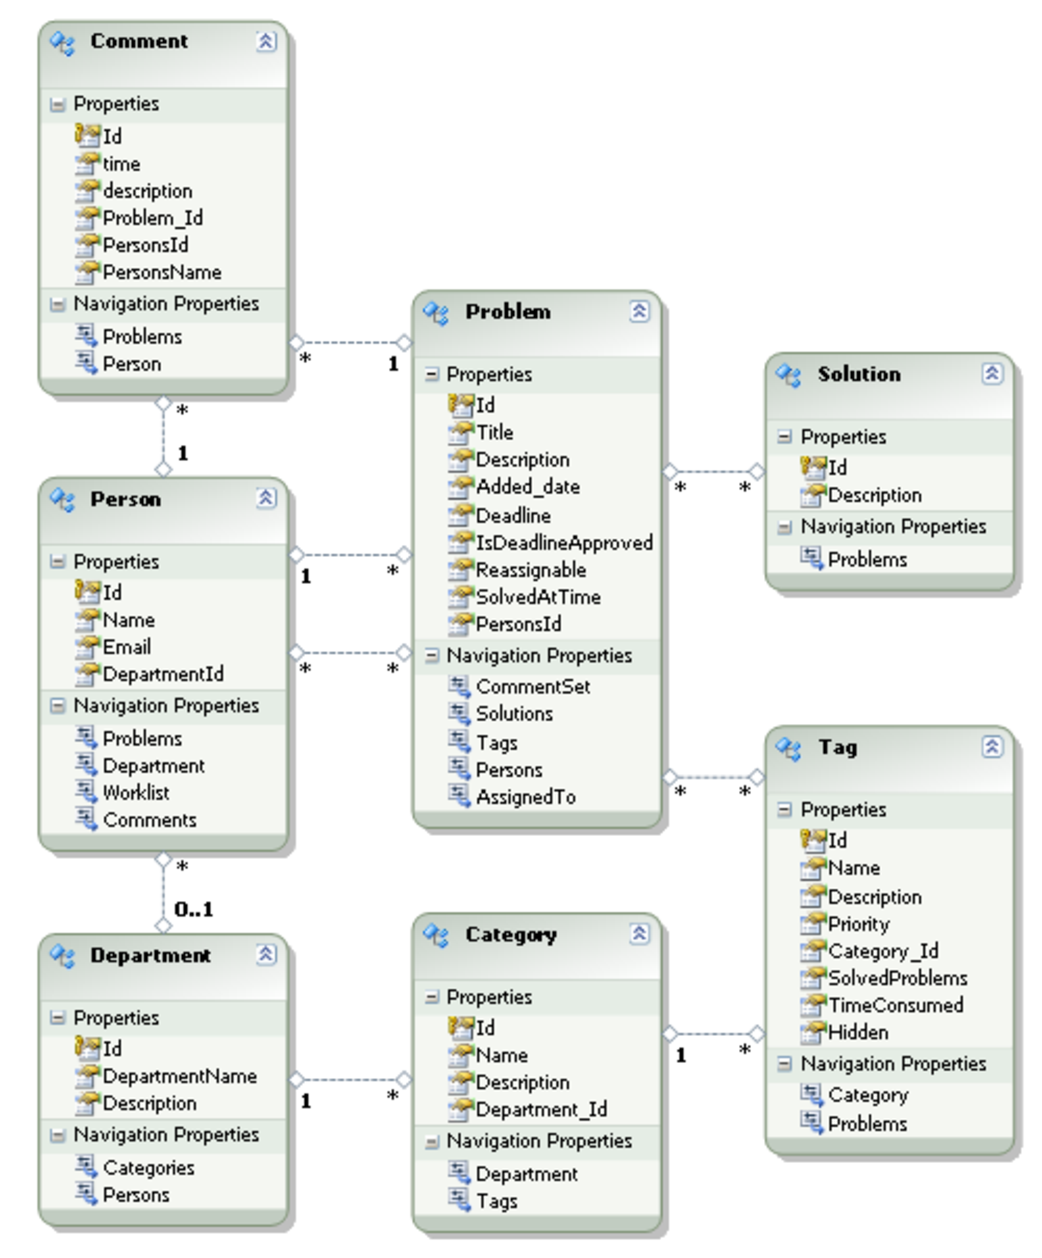
\includegraphics[scale=0.7]{input/implementation/mvc/Model.pdf}
	\morscaption{Our model as it is seen in the ADO.NET Entity Data Model Designer.}
	\label{fig:edmxModel}
\end{figure}
